%% State Space Modelling of Dynamic Systems
%% Lecture 21: State Observers
\def\FileDate{10/04/02}
\def\FileVersion{1.0}
% ----------------------------------------------------------------
% Notes pages *********************************************************
% ----------------------------------------------------------------

In many practical cases it is not possible to measure all the states of a system.
That is  we cannot form  $u=r-\mathbf{Kx}$  for the purposes of feedback control because we do not have access to $\mathbf{x}$\footnote{Or some states in $\mathbf{x}$, either because the states are not \emph{physical states} and hence cannot be measured, or because they \emph{are} physical states but we do not have suitable sensors for the physical quantity that is represented by the state.}

If the structure of the system is known  (i.e. $\mathbf{A}$, $\mathbf{B}$, $\mathbf{C}$, and $\mathbf{D}$) then it may be possible to reconstruct the states from one or more of the system outputs by means of an observer. It is necessary that the system states be observable from the output(s).

\ifslidesonly
\begin{slide}
   \heading{State Observers}
   \begin{itemize}
   	\item In many practical cases it is not possible to measure all the states of a system.
   	\item That is  we cannot form  $u=r-\mathbf{Kx}$  for the purposes of feedback control because we do not have access to $\mathbf{x}$.
   	\item If we know $\mathbf{A}$, $\mathbf{B}$, $\mathbf{C}$, and $\mathbf{D}$ then it may be possible to reconstruct the states from one or more of the system outputs by means of an \textbf{observer}. 
   	\item It is necessary that the system states be observable from the output(s).
   \end{itemize}
\end{slide}
\fi

\begin{slide}
   \heading{State Observer}
The main idea is to construct a model of the system and subject it to the same input:
\begin{center}
	\resizebox{200pt}{!}{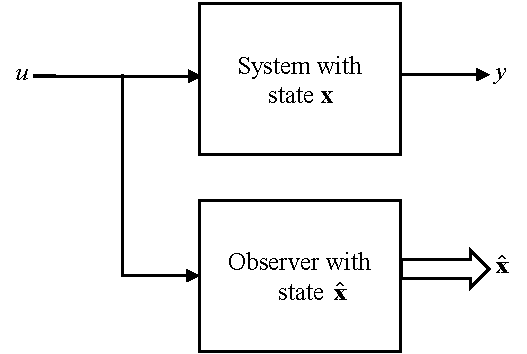
\includegraphics{pictures/observer1.pdf}}
\end{center}
\end{slide}

Severe differences occur between $\mathbf{x}$  and  $\hat{\mathbf{x}}$ due to disturbances and parameter errors. Solution:-  Employ feedback !

\begin{slide}
   \heading{State Observer with Feedback}
\begin{center}
	\resizebox{280pt}{!}{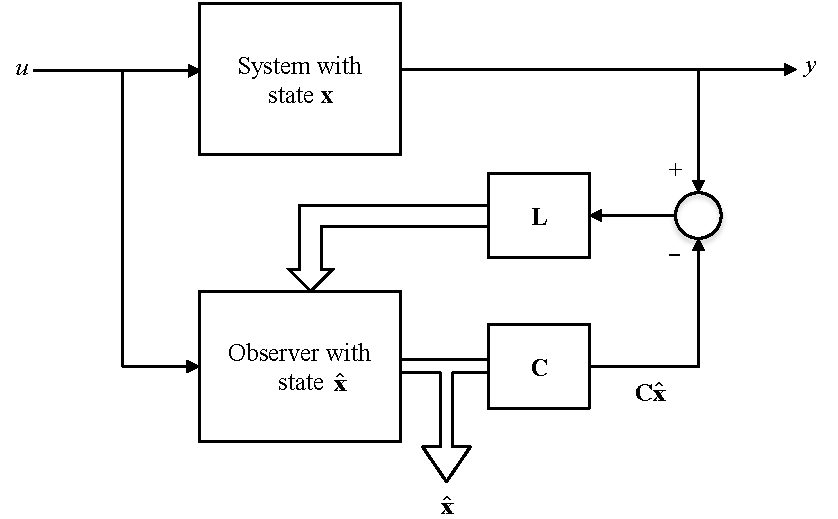
\includegraphics{pictures/observer2.pdf}}
\end{center}
\end{slide}
\textbf{NB} To simplify treatment, we take $\mathbf{D}=0$.


\begin{center}
	\resizebox{200pt}{!}{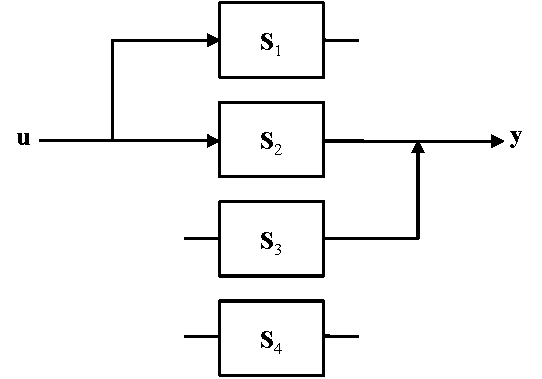
\includegraphics{pictures/partitioning.pdf}}
\end{center}
\endinput

%%% Local Variables: 
%%% mode: latex
%%% TeX-master: "notes"
%%% End:
\ifslidesonly
\begin{slide}
	\heading{Observer State Equations}
   
\begin{center}
	\resizebox{200pt}{!}{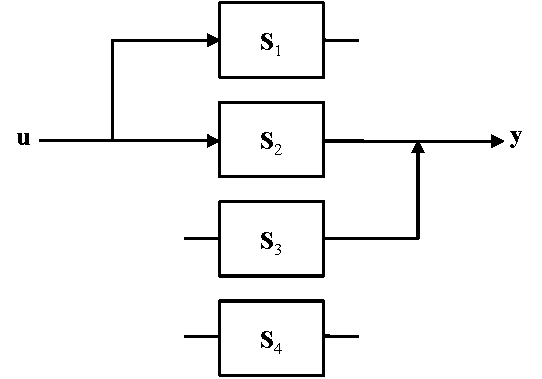
\includegraphics{pictures/partitioning.pdf}}
\end{center}
\endinput

%%% Local Variables: 
%%% mode: latex
%%% TeX-master: "notes"
%%% End:
\end{slide}
\fi


Given the transformation $\mathbf{T}^{-1}\mathbf{AT}=\mathbf{\Lambda}$:
\begin{eqnarray*}
	\mathbf{A}t & = & (\mathbf{T\Lambda T}^{-1}) t \\
	\mathbf{A}^nt^n & = & (\mathbf{T\Lambda T}^{-1})(\mathbf{T\Lambda T}^{-1})\ldots(\mathbf{T\Lambda T}^{-1})t^n \\
	                & = & \mathbf{T\Lambda T}^{-1}\mathbf{T\Lambda T}^{-1}\ldots\mathbf{T\Lambda T}^{-1}t^n \\
	\mathbf{A}^nt^n & = & \mathbf{T\Lambda}\mathbf{I}\mathbf{\Lambda I}\ldots\mathbf{I\Lambda T}^{-1}t^n \\
	\               & = & \mathbf{T\Lambda}^n\mathbf{T}^{-1}t^n \\
\end{eqnarray*}
\endinput

%%% Local Variables: 
%%% mode: latex
%%% TeX-master: "notes"
%%% End:
\ifslidesonly
\begin{slide}
	\heading{Observed State Errors}
   Given the transformation $\mathbf{T}^{-1}\mathbf{AT}=\mathbf{\Lambda}$:
\begin{eqnarray*}
	\mathbf{A}t & = & (\mathbf{T\Lambda T}^{-1}) t \\
	\mathbf{A}^nt^n & = & (\mathbf{T\Lambda T}^{-1})(\mathbf{T\Lambda T}^{-1})\ldots(\mathbf{T\Lambda T}^{-1})t^n \\
	                & = & \mathbf{T\Lambda T}^{-1}\mathbf{T\Lambda T}^{-1}\ldots\mathbf{T\Lambda T}^{-1}t^n \\
	\mathbf{A}^nt^n & = & \mathbf{T\Lambda}\mathbf{I}\mathbf{\Lambda I}\ldots\mathbf{I\Lambda T}^{-1}t^n \\
	\               & = & \mathbf{T\Lambda}^n\mathbf{T}^{-1}t^n \\
\end{eqnarray*}
\endinput

%%% Local Variables: 
%%% mode: latex
%%% TeX-master: "notes"
%%% End:
\end{slide}
\fi
 
The matrix function becomes:
\begin{eqnarray*}
	f(\mathbf{A}t) & = & f_0\mathbf{TIT}^{-1} + f_1\mathbf{T\Lambda T}^{-1}t + f_2\mathbf{T\Lambda}^2\mathbf{T}^{-1}t^2 + \cdots + f_n\mathbf{T\Lambda}^n\mathbf{T}^{-1}t^n + \cdots \\
	f(\mathbf{A}t) & = & \mathbf{T}\left(f_0\mathbf{I} + f_1\mathbf{\Lambda}t + f_2\mathbf{\Lambda}^2t^2 + \cdots + f_n\mathbf{\Lambda}^nt^n + \cdots \right)\mathbf{T}^{-1}\\
	               & = & \mathbf{T}f(\mathbf{\Lambda}t)\mathbf{T}^{-1}
\end{eqnarray*}
 
The term inside the brackets on the rhs is a diagonal matrix and the $i^\mathrm{th}$ diagonal element is:
\[
f_0+f_1\lambda_it + f_2\lambda_i^2t^2 + \cdots + f_n\lambda_i^nt^ + \cdots
\]
From the Taylor series this must be $f(\lambda_i t)$:
\[
f(\mathbf{A} t)=\mathbf{T} f(\mathbf{\Lambda} t) \mathbf{T}^{-1}
\]   
where $f(\mathbf{\Lambda} t)=\mathrm{diag}\left(f(\lambda_i t)\right)$.

\endinput

%%% Local Variables: 
%%% mode: latex
%%% TeX-master: "notes"
%%% End:
\ifslidesonly
\begin{slide}
	\heading{Properties of the Observed Error State Equations}
   The matrix function becomes:
\begin{eqnarray*}
	f(\mathbf{A}t) & = & f_0\mathbf{TIT}^{-1} + f_1\mathbf{T\Lambda T}^{-1}t + f_2\mathbf{T\Lambda}^2\mathbf{T}^{-1}t^2 + \cdots + f_n\mathbf{T\Lambda}^n\mathbf{T}^{-1}t^n + \cdots \\
	f(\mathbf{A}t) & = & \mathbf{T}\left(f_0\mathbf{I} + f_1\mathbf{\Lambda}t + f_2\mathbf{\Lambda}^2t^2 + \cdots + f_n\mathbf{\Lambda}^nt^n + \cdots \right)\mathbf{T}^{-1}\\
	               & = & \mathbf{T}f(\mathbf{\Lambda}t)\mathbf{T}^{-1}
\end{eqnarray*}
 
The term inside the brackets on the rhs is a diagonal matrix and the $i^\mathrm{th}$ diagonal element is:
\[
f_0+f_1\lambda_it + f_2\lambda_i^2t^2 + \cdots + f_n\lambda_i^nt^ + \cdots
\]
From the Taylor series this must be $f(\lambda_i t)$:
\[
f(\mathbf{A} t)=\mathbf{T} f(\mathbf{\Lambda} t) \mathbf{T}^{-1}
\]   
where $f(\mathbf{\Lambda} t)=\mathrm{diag}\left(f(\lambda_i t)\right)$.

\endinput

%%% Local Variables: 
%%% mode: latex
%%% TeX-master: "notes"
%%% End:
\end{slide}
\fi


\section*{Design of the $\mathbf{L}$ Matrix} % (fold)
\label{sec:design_of_the_l_matrix}

The vector $[v_{31}, i_{1}]^T$ is called the ``\emph{state
vector}.'' Its elements are state variables.
\endinput
%%% Local Variables: 
%%% mode: latex
%%% TeX-master: "notes"
%%% End: 

\ifslidesonly
\begin{slide}
	\heading{Design of the $\mathbf{L}$ Matrix (1)}
   The vector $[v_{31}, i_{1}]^T$ is called the ``\emph{state
vector}.'' Its elements are state variables.
\endinput
%%% Local Variables: 
%%% mode: latex
%%% TeX-master: "notes"
%%% End: 

\end{slide}
\fi

From previous work the error dynamics are:
\[
\dot{\mathbf{e}} = (\mathbf{A}-\mathbf{LC})\mathbf{e}
\]
Therefore the dynamics of the combined system is:
\[\left[ {\begin{array}{*{20}c}
   {\dot{\mathbf{x}}}  \\
   {\dot{\mathbf{e}}ß}  \\
\end{array}} \right] = \left[ {\begin{array}{*{20}c}
   {\left( {{\bf{A}} - {\bf{BK}}} \right)} & {{\bf{BK}}}  \\
   {\bf{0}} & {\left( {{\bf{A}} - {\bf{LC}}} \right)}  \\
\end{array}} \right]\left[ {\begin{array}{*{20}c}
   {\bf{x}}  \\
   {\bf{e}}  \\
\end{array}} \right] + \left[ {\begin{array}{*{20}c}
   {\bf{B}}  \\
   {\bf{0}}  \\
\end{array}} \right]r
\]
\endinput

%%% Local Variables: 
%%% mode: latex
%%% TeX-master: "notes"
%%% End:
\ifslidesonly
\begin{slide}
	\heading{Design of the $\mathbf{L}$ Matrix (2)}
   From previous work the error dynamics are:
\[
\dot{\mathbf{e}} = (\mathbf{A}-\mathbf{LC})\mathbf{e}
\]
Therefore the dynamics of the combined system is:
\[\left[ {\begin{array}{*{20}c}
   {\dot{\mathbf{x}}}  \\
   {\dot{\mathbf{e}}ß}  \\
\end{array}} \right] = \left[ {\begin{array}{*{20}c}
   {\left( {{\bf{A}} - {\bf{BK}}} \right)} & {{\bf{BK}}}  \\
   {\bf{0}} & {\left( {{\bf{A}} - {\bf{LC}}} \right)}  \\
\end{array}} \right]\left[ {\begin{array}{*{20}c}
   {\bf{x}}  \\
   {\bf{e}}  \\
\end{array}} \right] + \left[ {\begin{array}{*{20}c}
   {\bf{B}}  \\
   {\bf{0}}  \\
\end{array}} \right]r
\]
\endinput

%%% Local Variables: 
%%% mode: latex
%%% TeX-master: "notes"
%%% End:
\end{slide}
\fi

When the initial conditions of the state-variables are all zero,
this reduces to the transfer matrix model
\begin{equation}\label{eqn:transfer-function}
  \mathbf{Y}=\left[\mathbf{C}\left[s\mathbf{I}-\mathbf{A}\right]^{-1}\mathbf{B}+\mathbf{D}\right]\mathbf{U}
\end{equation}

\endinput

%%% Local Variables: 
%%% mode: latex
%%% TeX-master: "notes"
%%% End: 

\ifslidesonly
\begin{slide}
	\heading{Design of the $\mathbf{L}$ Matrix (3)}
   When the initial conditions of the state-variables are all zero,
this reduces to the transfer matrix model
\begin{equation}\label{eqn:transfer-function}
  \mathbf{Y}=\left[\mathbf{C}\left[s\mathbf{I}-\mathbf{A}\right]^{-1}\mathbf{B}+\mathbf{D}\right]\mathbf{U}
\end{equation}

\endinput

%%% Local Variables: 
%%% mode: latex
%%% TeX-master: "notes"
%%% End: 

\end{slide}
\fi


\subsection*{Example 1} % (fold)
\label{sub:example_1}

\textbf{Problem}: Design an observer with poles or eigen values $\lambda_{1,2} = -20,\ -20$ using the observer canonical form for the system with a TF:
\[
\frac{Y(s)}{U(s)}=\frac{7}{s^2+15s+44}.
\]
 
\textbf{SOLUTION}:
The observer canonical form gives:
% MathType!MTEF!2!1!+-
% faaagaart1ev2aaaKnaaaaWenf2ys9wBH5garuavP1wzZbqedmvETj
% 2BSbqefm0B1jxALjharqqtubsr4rNCHbGeaGqiVu0Je9sqqrpepC0x
% bbL8FesqqrFfpeea0xe9Lq-Jc9vqaqpepm0xbba9pwe9Q8fs0-yqaq
% pepae9pg0FirpepeKkFr0xfr-xfr-xb9Gqpi0dc9adbaqaaeGaciGa
% aiaabeqaamaabaabaaGcbaGaaCyqaiabg2da9maadmaabaqbamqabi
% GaaaqaaiabgkHiTiaaigdacaaI1aaabaGaaGymaaqaaiabgkHiTiaa
% isdacaaI0aaabaGaaGimaaaaaiaawUfacaGLDbaacaGG7aGaaGjbVl
% aahkeacqGH9aqpdaWadaqaauaadeqaceaaaeaacaaIWaaabaGaaG4n
% aaaaaiaawUfacaGLDbaacaGG7aGaaGjbVlaahoeacqGH9aqpdaWada
% qaauaadeqabiaaaeaacaaIXaaabaGaaGimaaaaaiaawUfacaGLDbaa
% caGG7aGaaGjbVlaahseacqGH9aqpcaaIWaaaaa!4C31!
\[
{\bf{A}} = \left[ {\begin{array}{*{20}c}
   { - 15} & 1  \\
   { - 44} & 0  \\
\end{array}} \right];\;{\bf{B}} = \left[ {\begin{array}{*{20}c}
   0  \\
   7  \\
\end{array}} \right];\;{\bf{C}} = \left[ {\begin{array}{*{20}c}
   1 & 0  \\
\end{array}} \right];\;{\bf{D}} = 0
\]
with $\mathbf{L}=[l_1,\ l_2]^T$  we have observer poles at the roots of:
\[
s^2+(15+l_1)s+(44+l_2)=0.
\]
 

The desired CE is:
\[
\alpha_e(s)=(s + 20)(s + 20)=s^2+40s+400=0
\]

Comparing coefficients gives:
\begin{eqnarray*}
	s^1:\ 15 + l_1 & = & 40 \to l_1=25 \\
	s^0:\ 44 + l_2 & = & 400 \to l_2=356 \\	
\end{eqnarray*}
 

So the observer states are given by:
\[
\frac{d\hat{\mathbf{x}}}{dt}=\mathbf{A}\hat{\mathbf{x}}+\mathbf{B}u-\mathbf{L}(\mathbf{C}\hat{\mathbf{x}}-y)
\]
where $\mathbf{L}=[25\ 356]^T.$

\begin{slide}
   \heading{Block Diagram of the Observer}
\begin{center}
	\resizebox{250pt}{!}{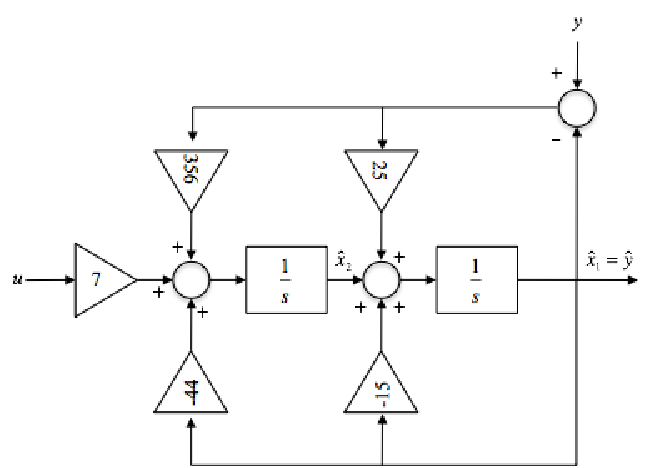
\includegraphics{pictures/observer3.pdf}}
\end{center}
\end{slide}

% subsection example_1 (end)

% section design_of_the_l_matrix (end)


\section*{Design of $\mathbf{L}$ Matrix for Other Forms of State Equation} % (fold)
\label{sec:design_of_l_matrix_for_other_forms_of_state_equation}


When the observer canonical form is not used, then the design of the observer is more difficult. Ackermann's formula can be adapted as follows:
% MathType!MTEF!2!1!+-
% faaagaart1ev2aaaKnaaaaWenf2ys9wBH5garuavP1wzZbqedmvETj
% 2BSbqefm0B1jxALjharqqtubsr4rNCHbGeaGqiVu0Je9sqqrpepC0x
% bbL8FesqqrFfpeea0xe9Lq-Jc9vqaqpepm0xbba9pwe9Q8fs0-yqaq
% pepae9pg0FirpepeKkFr0xfr-xfr-xb9Gqpi0dc9adbaqaaeGaciGa
% aiaabeqaamaabaabaaGcbaGaaCitamaaCaaaleqabaGaamivaaaaki
% abg2da9maadmaabaqbamqabeabaaaabaGaaGimaaqaaiablAcilbqa
% aiaaicdaaeaacaaIXaaaaaGaay5waiaaw2faaiaad+eadaahaaWcbe
% qaaiabgkHiTiaaigdaaaGccqaHXoqydaWgaaWcbaGaam4yaaqabaGc
% caGGOaGaaCyqamaaCaaaleqabaGaamivaaaakiaacMcaaaa!3EF6!
\[
{\bf{L}}^T  = \left[ {\begin{array}{*{20}c}
   0 &  \ldots  & 0 & 1  \\
\end{array}} \right]\mathcal{O}^{ - 1} \alpha _e ({\bf{A}}^T )
\]
$\mathcal{O}$ is the observability matrix:
\[
\mathcal{O}=[\mathbf{C}^T\vdots\mathbf{A}^T\mathbf{C}^T\vdots\cdots\vdots(\mathbf{A}^T)^{n-1}\mathbf{C}^T]
\]
and if $\alpha_e(s)=s^n + \alpha_1s^{n-1}+\cdots+\alpha_n$ then \[\alpha_e(\mathbf{A}^T)=(\mathbf{A}^T)^n + \alpha_1(\mathbf{A}^T)^{n-1}+\cdots+\mathbf{I}\alpha_n.\]
 

Notice that if the system is unobservable, then the matrix inverse $\mathcal{O}^{-1}$ does not exist and we cannot design an observer for this system.


 
 

\endinput

%%% Local Variables: 
%%% mode: latex
%%% TeX-master: "notes"
%%% End:
\ifslidesonly
\begin{slide}
	\heading{Design of $\mathbf{L}$ Matrix for Other Forms of State Equation}
   When the observer canonical form is not used, then the design of the observer is more difficult. Ackermann's formula can be adapted as follows:
% MathType!MTEF!2!1!+-
% faaagaart1ev2aaaKnaaaaWenf2ys9wBH5garuavP1wzZbqedmvETj
% 2BSbqefm0B1jxALjharqqtubsr4rNCHbGeaGqiVu0Je9sqqrpepC0x
% bbL8FesqqrFfpeea0xe9Lq-Jc9vqaqpepm0xbba9pwe9Q8fs0-yqaq
% pepae9pg0FirpepeKkFr0xfr-xfr-xb9Gqpi0dc9adbaqaaeGaciGa
% aiaabeqaamaabaabaaGcbaGaaCitamaaCaaaleqabaGaamivaaaaki
% abg2da9maadmaabaqbamqabeabaaaabaGaaGimaaqaaiablAcilbqa
% aiaaicdaaeaacaaIXaaaaaGaay5waiaaw2faaiaad+eadaahaaWcbe
% qaaiabgkHiTiaaigdaaaGccqaHXoqydaWgaaWcbaGaam4yaaqabaGc
% caGGOaGaaCyqamaaCaaaleqabaGaamivaaaakiaacMcaaaa!3EF6!
\[
{\bf{L}}^T  = \left[ {\begin{array}{*{20}c}
   0 &  \ldots  & 0 & 1  \\
\end{array}} \right]\mathcal{O}^{ - 1} \alpha _e ({\bf{A}}^T )
\]
$\mathcal{O}$ is the observability matrix:
\[
\mathcal{O}=[\mathbf{C}^T\vdots\mathbf{A}^T\mathbf{C}^T\vdots\cdots\vdots(\mathbf{A}^T)^{n-1}\mathbf{C}^T]
\]
and if $\alpha_e(s)=s^n + \alpha_1s^{n-1}+\cdots+\alpha_n$ then \[\alpha_e(\mathbf{A}^T)=(\mathbf{A}^T)^n + \alpha_1(\mathbf{A}^T)^{n-1}+\cdots+\mathbf{I}\alpha_n.\]
 

Notice that if the system is unobservable, then the matrix inverse $\mathcal{O}^{-1}$ does not exist and we cannot design an observer for this system.


 
 

\endinput

%%% Local Variables: 
%%% mode: latex
%%% TeX-master: "notes"
%%% End:
\end{slide}
\fi

In MATLAB we could evaluate the $\mathbf{L}$ matrix using:
\begin{verbatim}
	L=(acker(A',C',p))'
\end{verbatim}  where  \verb|p|  is a vector of desired observer poles.
 


% section design_of_l_matrix_for_other_forms_of_state_equation (end)

 
\section*{Choice of Observer Poles} % (fold)
\label{sec:choice_of_observer_poles}


\begin{itemize}
	\item Rule of thumb: observer poles can be faster than the controller poles (i.e. further from the origin) by a factor of 2 to 6. This makes the effect of the observer dynamics short-term and the overall response is dominated by the controller poles.
	\item If noise/disturbance is present this has an effect on the choice:
	\begin{description}
		\item[Process noise $w$:] $d\mathbf{x}/dt=\mathbf{Ax}+\mathbf{B}u+\mathbf{B}_1 w$
		\item[Sensor noise $v$:]  $y = \mathbf{C}x+v$
		\item[Observer:] $d\hat{\mathbf{x}}=\mathbf{A}\hat{\mathbf{x}}+\mathbf{B}u+\mathbf{L}(y-\mathbf{C}\hat{\mathbf{x}})$
		\item[Error $\mathbf{e}=\mathbf{x}-\hat{\mathbf{x}}$:] $d\mathbf{e}/dt=(\mathbf{A}-\mathbf{LC})\mathbf{e}+\mathbf{B}_1 w - \mathbf{L}v.$
	\end{description}
\end{itemize}

\endinput

%%% Local Variables: 
%%% mode: latex
%%% TeX-master: "notes"
%%% End:
\ifslidesonly
\begin{slide}
	\heading{Choice of Observer Poles (1)}
   \begin{itemize}
	\item Rule of thumb: observer poles can be faster than the controller poles (i.e. further from the origin) by a factor of 2 to 6. This makes the effect of the observer dynamics short-term and the overall response is dominated by the controller poles.
	\item If noise/disturbance is present this has an effect on the choice:
	\begin{description}
		\item[Process noise $w$:] $d\mathbf{x}/dt=\mathbf{Ax}+\mathbf{B}u+\mathbf{B}_1 w$
		\item[Sensor noise $v$:]  $y = \mathbf{C}x+v$
		\item[Observer:] $d\hat{\mathbf{x}}=\mathbf{A}\hat{\mathbf{x}}+\mathbf{B}u+\mathbf{L}(y-\mathbf{C}\hat{\mathbf{x}})$
		\item[Error $\mathbf{e}=\mathbf{x}-\hat{\mathbf{x}}$:] $d\mathbf{e}/dt=(\mathbf{A}-\mathbf{LC})\mathbf{e}+\mathbf{B}_1 w - \mathbf{L}v.$
	\end{description}
\end{itemize}

\endinput

%%% Local Variables: 
%%% mode: latex
%%% TeX-master: "notes"
%%% End:
\end{slide}
\fi

The last example had a system TF with no zeros. In this case it is easy to construct the equivalent classical controller. We had the feedback law:
\[
u=r-5x_1-156x_2
\]

Now $y=7x_2$ and $\dot{x}_2=x_1$ therefore $X_2(s)=Y(s)/7$ and $X_1(s)=sX_2(s)=sY(s)/7$. Therefore
\begin{eqnarray*}
	U(s) & = & R(s)-rX_1(s)-156X_2(s) \\
	& = & R(s) - \frac{1}{7}(5s+156)Y(s)
\end{eqnarray*}

\endinput

%%% Local Variables: 
%%% mode: latex
%%% TeX-master: "notes"
%%% End:
\ifslidesonly
\begin{slide}
	\heading{Choice of Observer Poles (2)}
   The last example had a system TF with no zeros. In this case it is easy to construct the equivalent classical controller. We had the feedback law:
\[
u=r-5x_1-156x_2
\]

Now $y=7x_2$ and $\dot{x}_2=x_1$ therefore $X_2(s)=Y(s)/7$ and $X_1(s)=sX_2(s)=sY(s)/7$. Therefore
\begin{eqnarray*}
	U(s) & = & R(s)-rX_1(s)-156X_2(s) \\
	& = & R(s) - \frac{1}{7}(5s+156)Y(s)
\end{eqnarray*}

\endinput

%%% Local Variables: 
%%% mode: latex
%%% TeX-master: "notes"
%%% End:
\end{slide}
\fi



% section choice_of_observer_poles (end)



%----------------------------------------------------------------
% The end of notes
% ----------------------------------------------------------------
\endinput

%%% Local Variables: 
%%% mode: latex
%%% TeX-master: t
%%% End: 
